\documentclass[10pt]{paper}
\usepackage{bm,amsmath,fullpage,graphicx,chngcntr}

\counterwithin{figure}{section}

\title{Regressions And Stuff}


\begin{document}

\maketitle

\section{Function Basis}
Consider a basic prediction problem where given an input, $x$, we wish to predict a value $y$ (e.g. predict income given GPA, or predict crime rate given temperature). We train on a sample of labeled data (a set of $(x,y)$ pairs) to find a function $f(x)$ that will give the expected $y$ for new inputs $x$.

One approach to this problem is to model $f$ as the linear combination of \emph{basis functions}. In other words, we manually choose functions $\phi_1(x), \dots, \phi_n(x)$ and algorithmically pick coefficients $c_1, \dots, c_n$, which we put together as
\begin{align*}bm
f(x) &= c_1 \phi_1(x) + \dots + c_n \phi_n(x).
\end{align*}
We can rewrite this with 
\begin{align*}
\bm{c} &= \begin{bmatrix} c_1 & \cdots & c_n \end{bmatrix} \\
\bm{\phi}(x) &= \begin{bmatrix} \phi_1(x) & \cdots & \phi_n(x) \end{bmatrix}
\end{align*}
so that 
\begin{align}
f(x) &= \bm{c} \cdot \bm{\phi}(x). \label{eq:predictor}
\end{align}

The choice of the basis functions is somewhat arbitrary and often depends on the problem domain. Common choices are monomials ($\phi_i(x) = x^i$) and sinusoidals ($\phi_i(x) = \sin(i \pi x)$).

As for the algorithm to pick the coefficient vector $\bm{c}$, we discuss three methods: \emph{linear regression}, \emph{ridge regression}, and \emph{LASSO} (least absolute shrinkage and selection operator). We devote one section to exploring each method in the next three sections.

Before moving on, we develop common notation to set up the algorithmic problem. Suppose we are given the training data as column vectors $\bm{x}$ and $\bm{y}$ of length $m$ and have chosen $n$ basis functions given by $\bm{\phi}$. We let $X = \bm{\phi}(\bm{x})$ be the $m$ by $n$ matrix where the $i$-th row is $\bm{\phi}(x_i)$ and $x_i$ is the $i$-th element of $\bm{x}$. Thus, we can roughly frame our algorithm's goal as finding a column vector $\bm{c}$ of size $n$ such that
\begin{align}
\bm{y} &\approx X \bm{c}, \label{eq:problem}
\end{align}
where $X$ and $\bm{y}$ are taken as inputs.

\section{Linear Regression}

Linear regression is a regression method that simply aims to minimize the square of the magnitude of the difference of the two sides of (\ref{eq:problem}):
\begin{align}
\left| \bm{y} - X \bm{c} \right|^2. \label{eq:sse}
\end{align}
The expression in (\ref{eq:sse}) is known as the \emph{sum of squares error}, or SSE, as it is the sum of the squares of the differences in predicted versus real $y$ values. 

One way to find the optimal $\bm{c}$ is to expand the expression and set its partial derivative with respect to $\bm{c}$ equal to zero. Doing so yields
\begin{align}
\bm{c} &= \left( X^T X \right)^{-1} X^T \bm{y}. \label{eq:linearclosed}
\end{align}
We refer to (\ref{eq:linearclosed}) as the closed form for $\bm{c}$.

Another way to find $\bm{c}$ is to perform gradient descent with SSE as the objective function of $\bm{c}$.

We will illustrate and contrast these methods with an example, and then show the effects of choosing a different function basis. Our example is generated by taking $\bm{x}$ as numbers from 0 to 1 at intervals of $0.1$ and 
\begin{align*}
\bm{y} &= \cos(\pi \bm{x}) + \cos(2 \pi \bm{x}) + \text{noise}.
\end{align*}

\subsection{Polynomials with Closed Form}

We use $\bm{\phi}$ of size $n+1$ whose components are monomials of order 0 through $n$ as our funciton basis. Using this to compute $X$ and evaluate the closed form, we can obtain $\bm{c}$. We view the results as a plot of the training data points, the generating curve (without noise), and the predictor $f(x) = \bm{c} \cdot \bm{\phi}(x)$. This is shown in Figure \ref{fig:poly} for several values of $n$.

\begin{figure}[ht!]
  \centering
  \label{fig:poly}
  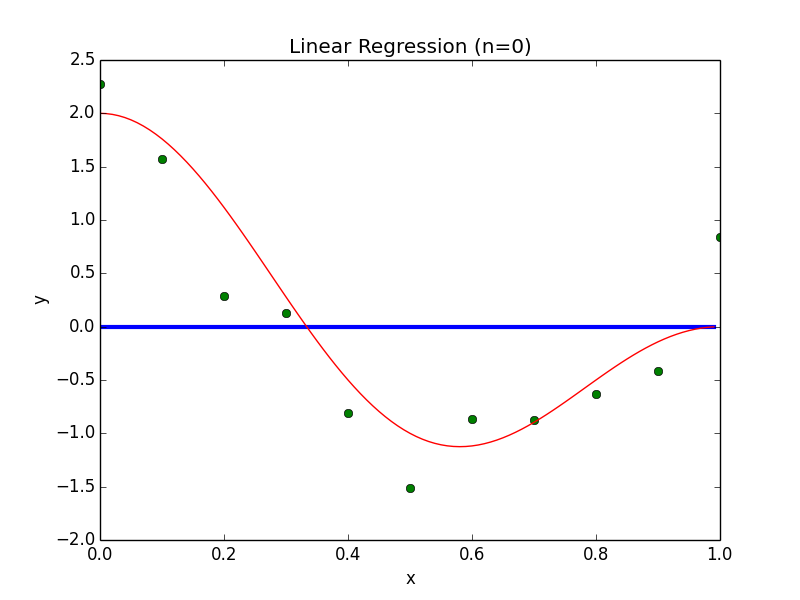
\includegraphics[width=0.45\textwidth]{../images/poly0.png}
  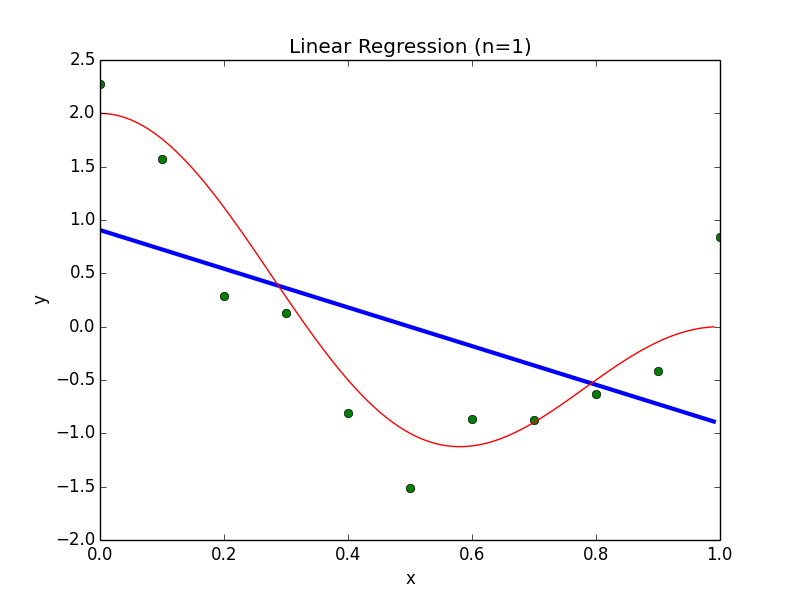
\includegraphics[width=0.45\textwidth]{../images/poly1.png}
  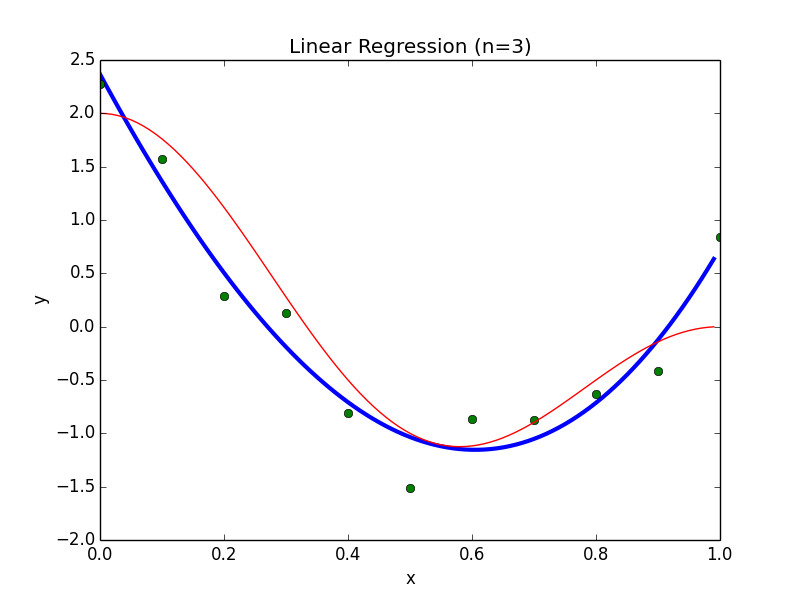
\includegraphics[width=0.45\textwidth]{../images/poly3.png}
  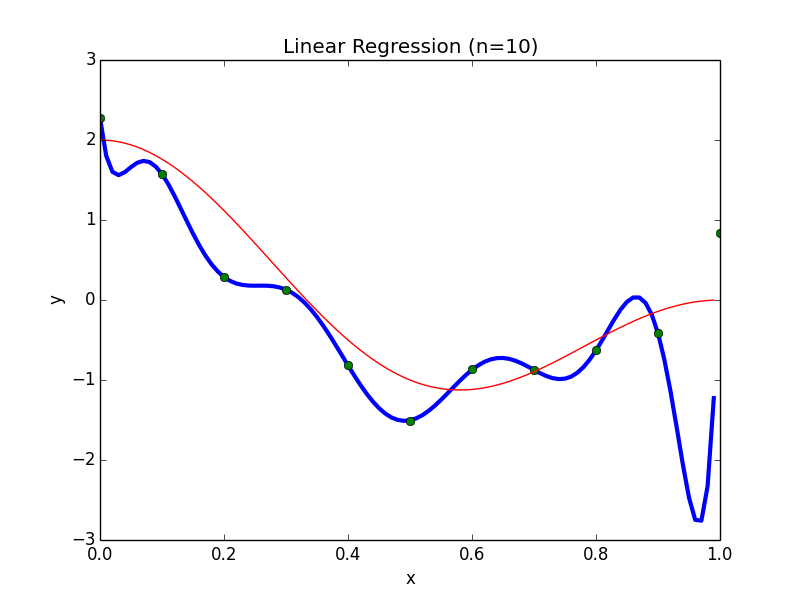
\includegraphics[width=0.45\textwidth]{../images/poly10.png}
  \caption{Training data (green), generating curve (red), and predicted curve (blue) for various $n$.}
\end{figure}

We can see that increasing the dimension of the function basis improves the training accuracy of our predictor.

\subsection{Polynomials with Gradient Descent}

Use batch gradient descent on the SSE function on some values of M. Describe your experience
with initial guesses, step sizes and convergence thresholds. Compare with using SGD on the
same data. Explain your results in terms of the properties of the function being optimized and
the properties of the algorithms.

\subsection{Cosines with Closed Form and Gradient Descent}

We now try using the function basis consisting of $\cos(\pi x), \cos(2 \pi x), \dots, \cos(n \pi x)$. In this case the closed form and both versions of gradient descent all give the same coefficient vectors after converging. We plot in Figure \ref{fig:cos} comparisons for a couple values of $n$.

\begin{figure}[ht!]
  \centering
  \label{fig:cos}
  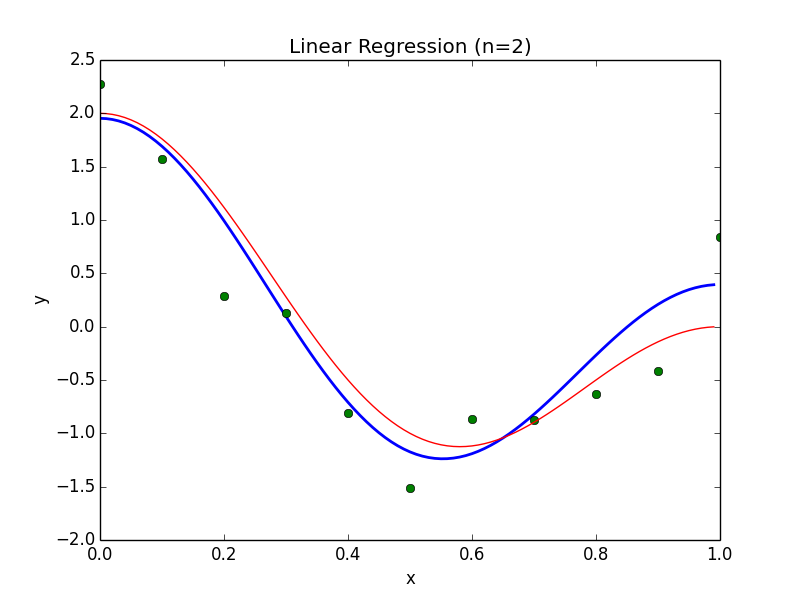
\includegraphics[width=0.45\textwidth]{../images/cos2.png}
  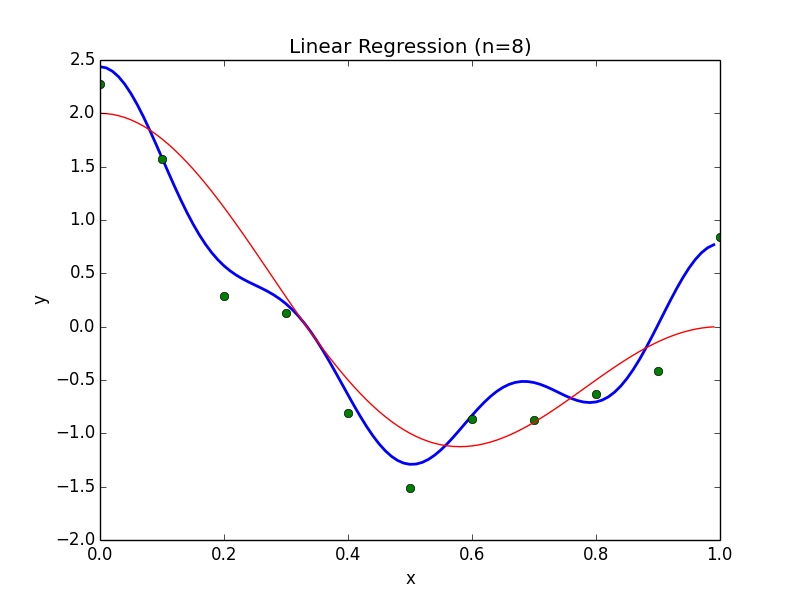
\includegraphics[width=0.45\textwidth]{../images/cos8.png}
  \caption{Training data (green), generating curve (red), and predicted curve (blue) for various $n$.}
\end{figure}

A notable observation is that even when the same basis functions were used as in the generating function ($\cos(\pi x)$ and $\cos(2\pi x)$ when $n=2$), we obtained a slightly different predicted curve. This is due to the added noise.

Also, when we increase the dimension of the basis ($n=8$) the predicted curve becomes more complex. Although it is more accurate for the training data, it is more sensitive to the noise and so wouldn't generalize well to new test data. This behavior is called \emph{overfitting}, which results when the coefficients become too large or when too many features (basis functions) are used. We will see below that these issues can be addressed using ridge regression and LASSO, respectively.

\section{Ridge Regression}

Ridge regression is similar to linear regression in that its choice of $\bm{c}$ aims to minimize SSE, but in addition also aims to minimize the size of the coefficients themselves. Tangibly, this is achieved by choosing $\bm{c}$ that gives the minimal value of
\begin{align}
\left| \bm{y} - X \bm{c} \right|^2 + \lambda \left| \bm{c} \right|^2. \label{eq:ridgeobjective}
\end{align}
We can tune the sensitivity to coefficient sizes by adjusting the parameter $\lambda$. At the extreme, $\lambda = 0$ will have no consideration of coefficient size and will be the same as linear regression.

Again, there are two ways to arrive at the desired $\bm{c}$ from here. First, we can expand (\ref{eq:ridgeobjective}) and set the partial derivative with respect to $\bm{c}$ equal to zero, which gives
\begin{align*}
\bm{c} &= \left( X^T X + \lambda I \right)^{-1} X^T \bm{y}. \label{eq:ridgeclosed}
\end{align*}
Second, we can perform gradient descent and converge to the optimal value of $\bm{c}$ numerically.

In general, the advantage of the second term in the objective function is that resulting coefficients are smaller, thus empirically less sensitive to noise and more accurate on unseen data.


\section{LASSO}



\end{document}

